\documentclass{beamer}
%SAND 2023-06062O
\usepackage{comment}
\usepackage{color}
\usepackage{listings}
\usepackage{verbatim}
\usepackage{multicol}
\usepackage{booktabs}
\definecolor{green}{RGB}{0,128,0}

\def\EQ#1\EN{\begin{equation*}#1\end{equation*}}
\def\BA#1\EA{\begin{align*}#1\end{align*}}
\def\BS#1\ES{\begin{split*}#1\end{split*}}
\newcommand{\bc}{\begin{center}}
\newcommand{\ec}{\end{center}}
\newcommand{\eq}{\ =\ }
\newcommand{\degc}{$^\circ$C}

\def\p{\partial}
\def\qbs{\boldsymbol{q}}
\def\Dbs{\boldsymbol{D}}
\def\A{\mathcal A}
\def\gC{\mathcal C}
\def\gD{\mathcal D}
\def\gL{\mathcal L}
\def\M{\mathcal M}
\def\P{\mathcal P}
\def\Q{\mathcal Q}
\def\gR{\mathcal R}
\def\gS{\mathcal S}
\def\X{\mathcal X}
\def\bnabla{\boldsymbol{\nabla}}
\def\bnu{\boldsymbol{\nu}}
\renewcommand{\a}{{\alpha}}
%\renewcommand{\a}{{}}
\newcommand{\s}{{\sigma}}
\newcommand{\bq}{\boldsymbol{q}}
\newcommand{\bz}{\boldsymbol{z}}
\def\bPsi{\boldsymbol{\Psi}}

\def\Li{\textit{L}}
\def\Fb{\textbf{f}}
\def\Jb{\textbf{J}}
\def\cb{\textbf{c}}

\def\Dt{\Delta t}
\def\tpdt{{t + \Delta t}}
\def\bpsi{\boldsymbol{\psi}}
\def\dbpsi{\delta \boldsymbol{\psi}}
\def\bc{\textbf{c}}
\def\dbc{\delta \textbf{c}}
\def\arrows{\rightleftharpoons}

\newcommand{\bGamma}{\boldsymbol{\Gamma}}
\newcommand{\bOmega}{\boldsymbol{\Omega}}
%\newcommand{\bPsi}{\boldsymbol{\Psi}}
%\newcommand{\bpsi}{\boldsymbol{\psi}}
\newcommand{\bO}{\boldsymbol{O}}
%\newcommand{\bnu}{\boldsymbol{\nu}}
\newcommand{\bdS}{\boldsymbol{dS}}
\newcommand{\bg}{\boldsymbol{g}}
\newcommand{\bk}{\boldsymbol{k}}
%\newcommand{\bq}{\boldsymbol{q}}
\newcommand{\br}{\boldsymbol{r}}
\newcommand{\bR}{\boldsymbol{R}}
\newcommand{\bS}{\boldsymbol{S}}
\newcommand{\bu}{\boldsymbol{u}}
\newcommand{\bv}{\boldsymbol{v}}
%\newcommand{\bz}{\boldsymbol{z}}
\newcommand{\pressure}{P}

\def\water{H$_2$O}
\def\calcium{Ca$^{2+}$}
\def\copper{Cu$^{2+}$}
\def\magnesium{Mg$^{2+}$}
\def\sodium{Na$^+$}
\def\potassium{K$^+$}
\def\uranium{UO$_2^{2+}$}
\def\hion{H$^+$}
\def\hydroxide{0H$^-$}
\def\bicarbonate{HCO$_3^-$}
\def\carbonate{CO$_3^{2-}$}
\def\cotwo{CO$_2$(aq)}
\def\chloride{Cl$^-$}
\def\fluoride{F$^-$}
\def\phosphoricacid{HPO$_4^{2-}$}
\def\nitrate{NO$_3^-$}
\def\sulfate{SO$_4^{2-}$}
\def\souotwooh{$>$SOUO$_2$OH}
\def\sohuotwocothree{$>$SOHUO$_2$CO$_3$}
\def\soh{$>$SOH}

\newcommand\gehcomment[1]{{{\color{orange} #1}}}
\newcommand\add[1]{{{\color{blue} #1}}}
\newcommand\remove[1]{\sout{{\color{red} #1}}}
\newcommand\codecomment[1]{{{\color{green} #1}}}
\newcommand\redcomment[1]{{{\color{red} #1}}}
\newcommand\bluecomment[1]{{{\color{blue} #1}}}
\newcommand\greencomment[1]{{{\color{green} #1}}}
\newcommand\magentacomment[1]{{{\color{magenta} #1}}}

\begin{comment}
\tiny
\scriptsize
\footnotesize
\small
\normalsize
\large
\Large
\LARGE
\huge
\Huge
\end{comment}

\begin{document}

\title{1D Multicontinuum Radionuclide Transport \ldots in a Nutshell}
\author{Rosie Leone}
\date{\today}

%\frame{\titlepage}


%-----------------------------------------------------------------------------
\section{Description of a 1D Radionuclide Multicontinuum Model}

\subsection{1D Multicontinuum Transport Model}

\frame{\frametitle{Description of 1D Radionuclide Multicontinuum Scenario}
The ``1D Multicontinuum Radionuclide Transport Model'' simulates solute transport of two radionuclides within a 10 m single fracture with matrix diffusion in a 1 m 1D matrix:
\begin{itemize}
  \item Problem domain: $10 \times 1 \times 1$ m ($x \times y \times z$)
  \item Grid resolution $0.1 \times 1 \times 1$ m ($100 \times$ 1 $\times$ 1 cells)
  \item Secondary domain: 1 m
  \item Secondary grid cells per primary: 20
  \item Radionuclide Behavior: Controlled by \redcomment{UFD\_DECAY}
  \item Total simulation time: 5000 days
\end{itemize}

}

%-----------------------------------------------------------------------------
%\frame{\frametitle{1D Tracer Multicontinuum Scenario Schematic}
%\begin{itemize}
%  \item Transport in fracture due to advection and dispersion
%  \item Transport in matrix due to diffusion only
%\end{itemize}

%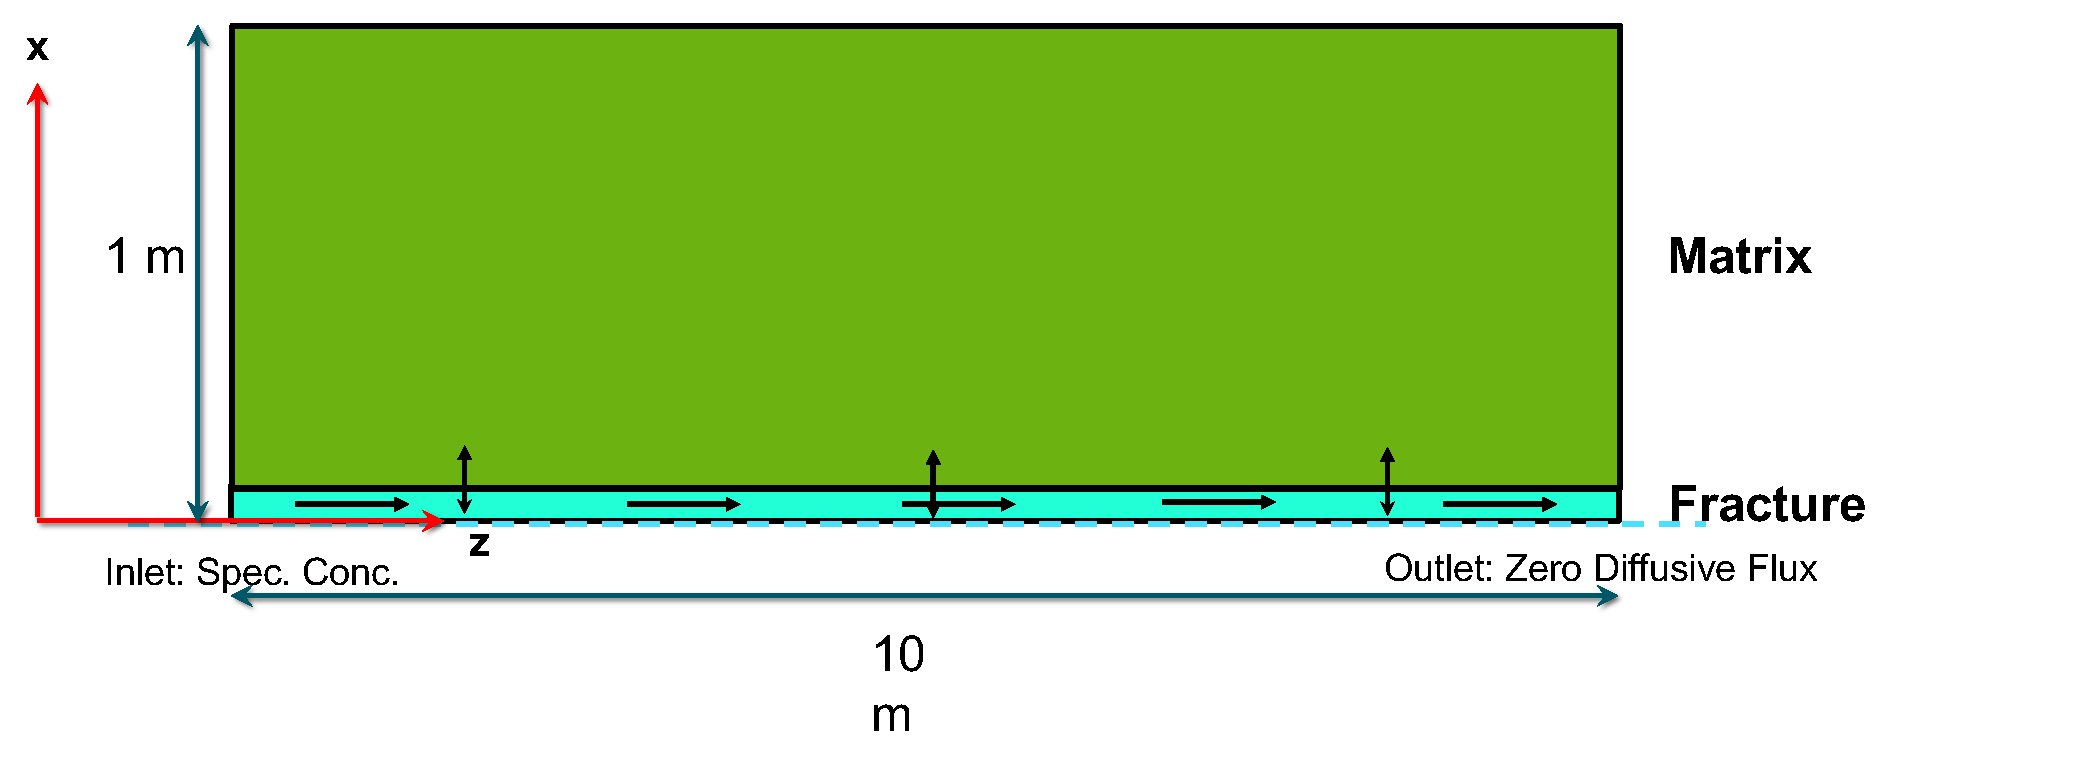
\includegraphics[width=\linewidth]{./slab_fig}
%}

%-----------------------------------------------------------------------------

\subsection{1D Multicontinuum Transport Model Steps}

\frame{\frametitle{Description of 1D Radionuclide Multicontinuum Scenario}
	The following tests will be run on the domain:
	\begin{itemize}
		\item Radionuclide transport without matrix diffusion (ufd\_nomc.in)
		\item Radionuclide transport with matrix diffusion (ufd\_mc.in)
		\item Radionuclide transport with matrix diffusion and decay (ufd\_mc\_decay.in)
		\item Radionuclide transport with matrix diffusion, decay, and sorption (ufd\_mc\_decay\_sorption.in)
	\end{itemize}
	
}
\subsection{Governing Equations
}
\frame{\frametitle{Governing Reactive Transport Equations}

%\Large

\EQ\label{primary}
\frac{\p}{\p t} \left(\varepsilon_f \varphi_f s \Psi_j^f\right) + \bnabla\cdot\bOmega_j^f \eq
-A_{fm} \bOmega_j^{fm} - \varepsilon_f \sum_k \nu_{jk} \Gamma_k^f 
\EN

\EQ\label{secondary}
\frac{\p}{\p t} \left(\varphi_m s \Psi_j^m\right) + \bnabla_\xi\cdot\bOmega_j^m \eq
- \sum_k \nu_{jk} \Gamma_k^m
\EN

\EQ\label{bc}
\bOmega_{j}^{fm} \left(x,t\right) = \bOmega_{j}^m \left(\xi_{fm},t\mid x\right)
\EN

\bigskip
\normalsize
\footnotesize
\begin{align*}
\varphi_f &\eq \text{porosity in fracture}; \quad
\varphi_m \eq \text{porosity in matrix}\\
\Psi &\eq \text{total component concentration}\\
\epsilon_f &\eq \text{Fracture volume fraction} \\
\bOmega &\eq \text{solute flux} \\
A_{fm} &\eq \text{fracture-matrix interfacial area} \\
\sum_k \nu_{jk} \Gamma_k^f &\eq \text{mineral reaction}\\
\xi &\eq \text{generalized one-dimensional coordinate} \\
x &\eq \text{point along fracture}; 
t \eq \text{time} 
\end{align*}

}
%-----------------------------------------------------------------------------
\subsection{Governing Equations}
\frame{\frametitle{UFD\_DECAY Governing Equations}
	
%\Large

\redcomment{Total mass [mol] of each isotope summed up according to,}
	
\EQ\label{totalmass}
M_i^{total} \eq M_i^{aq} + M_i^{sorb} + M_i^{ppt}
\EN

\redcomment{Mole fractions calculated to determine fraction each isotope contributes to total element mass}

\EQ\label{molefraction}
X_i \eq \frac{M_i^{total}}{M_e^{total}}
\EN

\redcomment{Element aqueous concentration calculated}

\EQ\label{aqconc}
C_e^{aq} \eq \frac{M_e^{total}}{1000 \left(1 + Kd_e / \left( \rho \phi S_l\right) \right) V\phi S_l}
\EN

}

%-----------------------------------------------------------------------------
\subsection{Governing Equations}
\frame{\frametitle{UFD\_DECAY Governing Equations}
	

\redcomment{Remaining element mass partitioned between sorbed and precipitated phases}

	\EQ\label{Csorb}
	C_e^{sorb} \eq C_e^{aq}Kd_e
	\EN
	
	\EQ\label{Cppt}
	C_e^{ppt} \eq \frac{M_e^{ppt}V_e^{mnrl}}{V}
	\EN
	
\redcomment{Isotope concentrations calculated from partitioned elemental concentrations}

	\EQ\label{Ci}
	C_i \eq X_iC_e
	\EN
}

%-----------------------------------------------------------------------------
\subsection{Governing Equations}
\frame{\frametitle{UFD\_DECAY Governing Equations}

\footnotesize
\begin{align*}
M_i^{aq} \eq \text{mass of isotope i in aqueous phase} \\
M_i^{sorb} \eq \text{mass of isotope i in sorbed phase} \\
M_i^{ppt} \eq \text{mass of isotope i in precipitated phase} \\
M_e^{total} \eq \text{total mass corresponding to element e}\\
X_i \eq \text{mass fraction for isotope i} \\
C_e^{aq} \eq \text{aqueous concentration} \\
C_e^{sorb} \eq \text{sorbed concentration}\\
C_e^{ppt} \eq \text{precipitated concentration}\\
Kd_e \eq \text{elemental Kd value}\\
\rho \eq \text{water density}\\
\phi \eq \text{material porosity}\\
S_l \eq \text{pore water saturation}\\
V_e^{mnrl} \eq \text{molar volume of precipitated element}\\
V \eq \text{grid cell volume}\\
\end{align*}	
	
	
	
}
%-----------------------------------------------------------------------------
\section{Description of Input Deck}

\subsection{SIMULATION}

\begin{frame}[fragile,containsverbatim]\frametitle{SIMULATION}

\begin{itemize}
  \item Radionuclide transport without matrix diffusion
\end{itemize}

\begin{semiverbatim}
SIMULATION
  SIMULATION_TYPE SUBSURFACE
  PROCESS_MODELS
    SUBSURFACE_TRANSPORT transport
      MODE GIRT
    /
    \magentacomment{UFD_DECAY ufd_decay !aqueous, solid, and sorbed phases
    /}  
  /
END

SUBSURFACE
  ...
END_SUBSURFACE
\end{semiverbatim}

\end{frame}

%-----------------------------------------------------------------------------
\begin{frame}[fragile,containsverbatim]\frametitle{GRID}

\begin{itemize}
  \item Problem domain: $10 \times 1 \times 1$ m (x $\times$ y $\times$ z)
  \item Grid resolution $100 \times 1 \times 1$ cells
\end{itemize}

\begin{semiverbatim}
GRID
  TYPE structured
  NXYZ 100 1 1
  BOUNDS
    0.d0 0.d0 0.d0
    10.d0 1.d0 1.d0
  /
END
\end{semiverbatim}

\end{frame}

%-----------------------------------------------------------------------------
\subsection{REGION}

\begin{frame}[fragile,containsverbatim,allowframebreaks]\frametitle{REGION}

\begin{itemize}
  \item Delineate regions for:
  \begin{itemize}
    \item entire domain
    \item west boundary face
    \item east boundary face
  \end{itemize}
\end{itemize}

\begin{semiverbatim}
REGION all
  COORDINATES
    0.d0  0.d0 0.d0
    10.d0 1.d0 1.d0
  /
END

\newpage
REGION west        \bluecomment{inflow of domain}
  FACE WEST
  COORDINATES
    0.d0 0.d0 0.d0
    0.d0 1.d0 1.d0
  /
END

REGION east           \bluecomment{outflow of domain}
  FACE EAST
  COORDINATES
    10.d0 0.d0 0.d0
    10.d0 1.d0 1.d0
  /
END
\end{semiverbatim}

\end{frame}


%-----------------------------------------------------------------------------
\subsection{MATERIAL\_PROPERTY}

\begin{frame}[fragile,containsverbatim]\frametitle{MATERIAL\_PROPERTY}

\begin{itemize}
  \item No secondary continuum
\end{itemize}

\begin{semiverbatim}
MATERIAL_PROPERTY soil1
  ID 1  
  POROSITY 5.d-5  \bluecomment{!fracture volume fraction}
  TORTUOSITY 0.2d0
  ROCK_DENSITY 2700.d0 #kg/m3
  LONGITUDINAL_DISPERSIVITY 0.5 #m
END
\end{semiverbatim}

\end{frame}

%-----------------------------------------------------------------------------
\subsection{FLUID\_PROPERTY}

\begin{frame}[fragile,containsverbatim]\frametitle{FLUID\_PROPERTY}

\begin{itemize}
  \item Assign a molecular diffusion coefficient of $10^{-9}$ m$^2$/s
\end{itemize}

\begin{semiverbatim}

FLUID_PROPERTY
  DIFFUSION_COEFFICIENT 1.d-9   \bluecomment{! [m^2/s]}
END
\end{semiverbatim}

\end{frame}

%-----------------------------------------------------------------------------
\subsection{CHEMISTRY}

\begin{frame}[fragile,allowframebreaks]\frametitle{CHEMISTRY}

\begin{itemize}
\item Aqueous and solid phase for each radionuclide
\end{itemize}

\begin{semiverbatim}
CHEMISTRY
  PRIMARY_SPECIES
    Am241
    Np237
  /
  MINERALS
    Am241(s)
    Np237(s)
  /
\end{semiverbatim}


\newpage

\begin{semiverbatim}
  MINERAL_KINETICS
    Am241(s)
      RATE_CONSTANT 0.d0
    /
    Np237(s)
      RATE_CONSTANT 0.d0
    /
  /    
  LOG_FORMULATION
  DATABASE ./ufd_decay.dat
  OUTPUT
    All
    TOTAL
  /
END
\end{semiverbatim}

\end{frame}

%-----------------------------------------------------------------------------
\subsection{Miscellaneous}

\begin{frame}[fragile]\frametitle{Miscellaneous}

\begin{itemize}
\item Specify a uniform Darcy velocity of 5e-7 m/d in the x-direction
\end{itemize}


\begin{semiverbatim}

SPECIFIED_VELOCITY
  UNIFORM? YES
  DATASET 5d-7 0.d0 0.d0 m/d
END
\end{semiverbatim}

\end{frame}


%-----------------------------------------------------------------------------
\subsection{TRANSPORT\_CONDITION / CONSTRAINT}

\begin{frame}[fragile,allowframebreaks]\frametitle{TRANSPORT\_CONDITION / CONSTRAINT}

\begin{itemize}
  \item Set up intial condition and inlet boundary condition
\end{itemize}

{
\begin{semiverbatim}

TRANSPORT_CONDITION initial
  TYPE DIRICHLET
  CONSTRAINT_LIST       \bluecomment{! list of constraints}
    0.d0 initial  
  /
END

TRANSPORT_CONDITION inlet      
  TYPE DIRICHLET
  CONSTRAINT_LIST       \bluecomment{! list of constraints}
    0.d0 inlet  
  /
END
\end{semiverbatim}
}

\newpage
{\small
\begin{semiverbatim}

TRANSPORT_CONDITION outlet      
  TYPE ZERO_GRADIENT
  CONSTRAINT_LIST       \bluecomment{! list of constraints}
    0.d0 initial  
  /
END
	
CONSTRAINT initial
  CONCENTRATIONS
    Am241  1.d-7  T 
    Np237  3.9d-9  T 
  /
  MINERALS
    Am241(s) 0.d0 1.d0
    Np237(s) 0.d0 1.d0
  /
/
\end{semiverbatim}
}

\newpage
{
	\begin{semiverbatim}
		
CONSTRAINT inlet
  CONCENTRATIONS
    Am241  4.d-7  T 
    Np237  1.0d-12  T 
  /
  MINERALS
    Am241(s) 0.d0 1.d0
    Np237(s) 0.d0 1.d0
  /
/


\end{semiverbatim}
}

\end{frame}




%-----------------------------------------------------------------------------
\subsection{INITIAL\_CONDITION}

\begin{frame}[fragile]\frametitle{INITIAL\_CONDITION}

\begin{itemize}
\item Couple the \greencomment{initial} transport conditions with region \greencomment{all} for the initial condition
\end{itemize}

\begin{semiverbatim}

INITIAL_CONDITION initial
  TRANSPORT_CONDITION initial
  REGION all
END

\end{semiverbatim}

\end{frame}

%-----------------------------------------------------------------------------
\subsection{BOUNDARY\_CONDITION}

\begin{frame}[fragile,allowframebreaks]\frametitle{BOUNDARY\_CONDITION}

\small
\begin{semiverbatim}
BOUNDARY_CONDITION inflow
  TRANSPORT_CONDITION inlet
  REGION west
END

BOUNDARY_CONDITION outflow
  TRANSPORT_CONDITION outlet
  REGION east
END

\end{semiverbatim}

\end{frame}

%-----------------------------------------------------------------------------
\subsection{TIME}

\begin{frame}[fragile]\frametitle{TIME}

\begin{itemize}
\item Set final simulation time to 5000 days
\item Set initial time step size to 1.e-3 days
\item Set maximum time step size to 1.0 days
\end{itemize}


\begin{semiverbatim}

TIME
  FINAL_TIME 5000.d0 d
  INITIAL_TIMESTEP_SIZE 1.d-3 d
  MAXIMUM_TIMESTEP_SIZE 1.d0 d
END
\end{semiverbatim}

\end{frame}

%-----------------------------------------------------------------------------
\subsection{OUTPUT}

\begin{frame}[fragile]\frametitle{OUTPUT}

\begin{itemize}
\item Print entire solution (a snapshot) in Tecplot format at specified times

\end{itemize}

\begin{semiverbatim}\small

OUTPUT
  SNAPSHOT_FILE
    FORMAT TECPLOT POINT
    TIMES d 800. 1100. 1140. 1180. 
  /
END

\end{semiverbatim}

\end{frame}
%-----------------------------------------------------------------------------
\subsection{STRATA}

\begin{frame}[fragile]\frametitle{STRATA}
	
\begin{itemize}
\item Couple material types with regions
\end{itemize}
	
\begin{semiverbatim}
STRATA
  REGION all
  MATERIAL soil1
END
		
\end{semiverbatim}
	
\end{frame}


%-----------------------------------------------------------------------------
\subsection{END\_SUBSURFACE}

\begin{frame}[fragile]\frametitle{END\_SUBSURFACE}
	
\begin{itemize}
\item Closes the SUBSURFACE block
\end{itemize}
	
\begin{semiverbatim}
END_SUBSURFACE
		
\end{semiverbatim}
	
\bluecomment{! UFD\_DECAY to follow}
\end{frame}
%-----------------------------------------------------------------------------
\subsection{UFD\_DECAY}

\begin{frame}[fragile]\frametitle{UFD\_DECAY}
	
\begin{itemize}
\item Solubility limits and sorption coefficients for each element
\end{itemize}
	
\begin{semiverbatim}
UFD_DECAY
  IMPLICIT_SOLUTION
  ELEMENT Am
    SOLUBILITY 4.d-7 \bluecomment{!mol/L}
    KD \bluecomment{! kg water / m^3 bulk}
      soil1 0.d0
    /
  /
  Element Np
    SOLUBILITY 4.d-9
    KD \bluecomment{! kg water / m^3 bulk}
      soil1 0.d0
    /
  /
		
\end{semiverbatim}
	
\end{frame}
%-----------------------------------------------------------------------------

%-----------------------------------------------------------------------------
\subsection{UFD\_DECAY}

\begin{frame}[fragile]\frametitle{UFD\_DECAY}
	
\begin{itemize}
\item Decay rates for each isotope
\end{itemize}
	
\begin{semiverbatim}
ISOTOPE Am241
  ELEMENT Am
  DECAY_RATE 0.d0 \bluecomment{!1/s}
/
ISOTOPE Np237
  ELEMENT Np
  DECAY_RATE 0.d0
/

END  \bluecomment{! UFD_DECAY}
		
\end{semiverbatim}
	
\end{frame}
%-----------------------------------------------------------------------------

\subsection{Running PFLOTRAN}

\begin{frame}[fragile]\frametitle{Running PFLOTRAN}

\begin{semiverbatim}

> cd $PFLOTRAN_DIR
> cd shortcourse/exercises/1D_tracer_multicontinuum/ufd
> pflotran -input_prefix ufd_nomc
> python concentration_ufd_nomc.py

\end{semiverbatim}

\end{frame}

%-----------------------------------------------------------------------------
\section{Description of Input Deck: Add matrix diffusion}

\subsection{Input File Modifications}

\begin{frame}[fragile]\frametitle{Add in matrix diffusion and secondary continuum}

Input File Modifications
\begin{itemize}
\item Modify cards:
  \begin{itemize}
    \item SIMULATION
    \item MATERIAL\_PROPERTIES
    \item OUTPUT
    \item REGION
    \item OBSERVATION
    \item UFD\_DECAY
   \end{itemize}
\end{itemize}

\end{frame}

%-----------------------------------------------------------------------------
\subsection{SIMULATION}

\begin{frame}[fragile,containsverbatim]\frametitle{SIMULATION}
	
	\begin{itemize}
		\item Add secondary continuum
	\end{itemize}
	
\begin{semiverbatim}
SIMULATION
  SIMULATION_TYPE SUBSURFACE
  PROCESS_MODELS
    SUBSURFACE_TRANSPORT transport
      MODE GIRT
      \magentacomment{OPTIONS
         MULTIPLE_CONTINUUM
       /}
    /
    UFD_DECAY ufd_decay
    /
  /
END
		
SUBSURFACE
...
END_SUBSURFACE
\end{semiverbatim}
	
\end{frame}

%-----------------------------------------------------------------------------
\subsection{MATERIAL\_PROPERTY}

\begin{frame}[fragile]\frametitle{MATERIAL\_PROPERTY}

\begin{itemize}
\item Add in secondary continuum to material
\end{itemize}

	
\begin{semiverbatim}
MATERIAL_PROPERTY soil1
ID 1
POROSITY \magentacomment{1.d0}
TORTUOSITY 1.d0
ROCK_DENSITY 2700.d0 #kg/m3
LONGITUDINAL_DISPERSIVITY 0.5 #m
\magentacomment{SECONDARY_CONTINUUM
  TYPE SLAB               \bluecomment{! single fracture}
  LENGTH 1.0              \bluecomment{! half fracture spacing [m]}
  NUM_CELLS 20            \bluecomment{! secondary cells per primary}
  EPSILON 0.00005d0       \bluecomment{! fracture volume fraction}
  LIQUID_DIFFUSION_COEFFICIENT 1.6d-10\bluecomment{!includes tortuosity}
  POROSITY 0.01           \bluecomment{! matrix porosity}
/ }
END
\end{semiverbatim}
	

\end{frame}

%-----------------------------------------------------------------------------
\subsection{OUTPUT}

\begin{frame}[fragile]\frametitle{OUTPUT}
	
	\begin{itemize}
		\item Add observation point
		
	\end{itemize}
	
	\begin{semiverbatim}\small
	\magentacomment{REGION obs
	  COORDINATE 1.0 0.5 0.5
	END}
	
	\magentacomment{OBSERVATION obs
	  REGION obs
	  SECONDARY_CONCENTRATION
	END}
		
	OUTPUT
	  SNAPSHOT_FILE
	    FORMAT TECPLOT POINT
	    TIMES d 800. 1100. 1140. 1180. 
	  /	
	  \magentacomment{OBSERVATION_FILE
	    PERIODIC TIMESTEP 1
	    PRINT_COLUMN_IDS
	  /}
	END
		
	\end{semiverbatim}
	
\end{frame}

%-----------------------------------------------------------------------------
\subsection{UFD\_DECAY}

\begin{frame}[fragile]\frametitle{UFD\_DECAY}
	
	\begin{itemize}
		\item Add secondary sorption coefficients for each element
	\end{itemize}
	
	\begin{semiverbatim}
UFD_DECAY
  IMPLICIT_SOLUTION
  ELEMENT Am
    SOLUBILITY 4.d-7 \bluecomment{!mol/L}
    KD \bluecomment{! kg water / m^3 bulk}
    \bluecomment{! first value primary kd, second value secondary kd}
      soil1 0.d0 \magentacomment{0.d0} 
    /
  /
  Element Np
    SOLUBILITY 4.d-9
    KD \bluecomment{! kg water / m^3 bulk}
    \bluecomment{! first value primary kd, second value secondary kd}
      soil1 0.d0 \magentacomment{0.d0}
    /
  /
		
	\end{semiverbatim}
	
\end{frame}

%-----------------------------------------------------------------------------

\subsection{Running PFLOTRAN}

\begin{frame}[fragile]\frametitle{Running PFLOTRAN}

\begin{semiverbatim}


> pflotran -input_prefix ufd_mc
> python concentration_ufd_mc.py

\end{semiverbatim}

\end{frame}

%-----------------------------------------------------------------------------
\section{Description of Input Deck: Add in decay}

\subsection{Input File Modifications}

\begin{frame}[fragile]\frametitle{Add in decay}
	
	Input File Modifications
	\begin{itemize}
		\item Modify cards:
		\begin{itemize}
			\item UFD\_DECAY
		\end{itemize}
	\end{itemize}
	
\end{frame}

%-----------------------------------------------------------------------------
\subsection{UFD\_DECAY}

\begin{frame}[fragile]\frametitle{UFD\_DECAY}
	
	\begin{itemize}
		\item Decay rates for each isotope
	\end{itemize}
	
	\begin{semiverbatim}
ISOTOPE Am241
  ELEMENT Am
    DECAY_RATE \magentacomment{5.08d-11} \bluecomment{!1/s}
      \magentacomment{DAUGHTER Np237 1.d0}
    /
ISOTOPE Np237
  ELEMENT Np
    DECAY_RATE \magentacomment{1.03d-14}
  /		
END  \bluecomment{! UFD_DECAY}
		
	\end{semiverbatim}
	
\end{frame}
%-----------------------------------------------------------------------------

\subsection{Running PFLOTRAN}

\begin{frame}[fragile]\frametitle{Running PFLOTRAN}
	
	\begin{semiverbatim}
		
		
		> pflotran -input_prefix ufd_mc_decay
		> python concentration_ufd_mc_decay.py
		
	\end{semiverbatim}
	
\end{frame}

%-----------------------------------------------------------------------------
\section{Description of Input Deck: Add in sorption}

\subsection{Input File Modifications}

\begin{frame}[fragile]\frametitle{Add in sorption}
	
	Input File Modifications
	\begin{itemize}
		\item Modify cards:
		\begin{itemize}
			\item UFD\_DECAY
		\end{itemize}
	\end{itemize}
	
\end{frame}


%-----------------------------------------------------------------------------
\subsection{UFD\_DECAY}

\begin{frame}[fragile]\frametitle{UFD\_DECAY}
	
	\begin{itemize}
		\item Add in kd values
	\end{itemize}
	
	\begin{semiverbatim}
UFD_DECAY
  IMPLICIT_SOLUTION
  ELEMENT Am
    SOLUBILITY 4.d-7 \bluecomment{!mol/L}
    KD \bluecomment{! kg water / m^3 bulk}
    \bluecomment{! add in kd value of secondary continuum}
      soil1 0.d0 \magentacomment{1.075d2}
    /
  /
  Element Np
    SOLUBILITY 4.d-9
    KD \bluecomment{! kg water / m^3 bulk}
    \bluecomment{! add in kd value of secondary continuum}
      soil1 0.d0 \magentacomment{5.37d3}
    /
  /
		
	\end{semiverbatim}
	
\end{frame}

%-----------------------------------------------------------------------------

\subsection{Running PFLOTRAN}

\begin{frame}[fragile]\frametitle{Running PFLOTRAN}
	
	\begin{semiverbatim}
		
		
		> pflotran -input_prefix ufd_mc_decay_sorption
		> python concentration_ufd_mc_decay_sorption.py
		
	\end{semiverbatim}
	
\end{frame}

\begin{frame}[fragile]
        
                Sandia National Laboratories is a multimission laboratory managed and operated by National Technology \& Engineering Solutions of Sandia, LLC, a wholly owned subsidiary of Honeywell International Inc., for the U.S. Department of Energy’s National Nuclear Security Administration under contract DE-NA0003525.

\end{frame}

\end{document}
